\chapter{Marcação de Parágrafos}
As classes padrão normalmente definem parágrafos recuados e sem nenhum espaço vertical entre parágrafos. Esta é a melhor solução ao usar um layout de página regular como os produzidos com o pacote \textbf{typearea}. Se nem recuo nem espaço vertical forem usados, apenas o comprimento da última linha daria ao leitor um guia para a quebra de parágrafo. Em casos extremos, é muito difícil dizer se uma linha está cheia ou não. Além disso, os tipógrafos descobrem que um sinal dado no final do parágrafo é facilmente esquecido no início da próxima linha. Um sinal no início do parágrafo é mais facilmente lembrado. O espaçamento entre parágrafos tem a desvantagem de desaparecer em alguns contextos. Por exemplo, após uma fórmula exibida, seria impossível detectar se o parágrafo anterior continua ou se um novo começa. Além disso, no topo de uma nova página, pode ser necessário olhar para a página anterior para determinar se um novo parágrafo foi iniciado ou não. Todos esses problemas desaparecem ao usar recuo. \textbf{Uma combinação de recuo e espaçamento vertical entre parágrafos é redundante e, portanto, deve ser evitada. O recuo por si só é suficiente. A única desvantagem do recuo é que ele encurta o comprimento da linha. O uso do espaçamento entre parágrafos é, portanto, justificado ao usar linhas curtas, como em um jornal.}

\section{parskip=method}
De vez em quando, você pode precisar de um layout de documento com espaçamento vertical entre parágrafos em vez de recuo. As classes \KOMAScript\ fornecem várias maneiras de fazer isso com a opção parskip. \textbf{O método consiste em dois elementos}. O primeiro elemento é \texttt{full} ou \texttt{half}, onde \texttt{full} representa um espaçamento de parágrafo de uma linha e \texttt{half} representa um espaçamento de parágrafo de meia linha. O segundo elemento consiste em um dos caracteres ``$\ast$'', ``$+$'' ou ``$-$'' e pode ser omitido. Sem o segundo elemento, a linha final de um parágrafo terminará com um espaço em branco de pelo menos 1em. Com o caractere ``$+$'' como o segundo elemento, o espaço em branco terá pelo menos um terço --- e com o asterisco um quarto --- da largura de uma linha normal. Com a variante menos, nenhuma provisão é feita para espaço em branco na última linha de um parágrafo.

Você pode alterar a configuração a qualquer momento. Se você alterá-la dentro do documento, o comando \char`\\\texttt{se\-lect\-font} será chamado implicitamente. Alterações no espaçamento de parágrafos dentro de um parágrafo não serão visíveis até o final do parágrafo.

Além das oito combinações resultantes para o método, você pode usar os valores para interruptores simples mostrado na tabela \ref{fig:8_1}, p.~\pageref{fig:8_1}. Ativar a opção \texttt{full} sem segundo elemento, portanto, resulta em espaçamento entre parágrafos de uma linha com pelo menos 1em de espaço em branco no final da última linha de cada parágrafo. Desativar a opção reativa o recuo padrão de 1em na primeira linha do parágrafo em vez do espaçamento de parágrafo. Um resumo de todos os valores possíveis para o método é mostrado na tabela \ref{fig:tab3_7}.

\begin{figure}[ht]
    \centering
    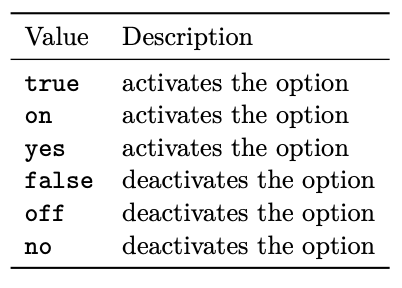
\includegraphics[width=0.5\linewidth]{arquivos/tab2_5.png}
    \caption{Valores padrão para interruptores simples em KOMA-Script}
    \label{fig:8_1}
\end{figure}

\begin{figure}[ht]
    \centering
    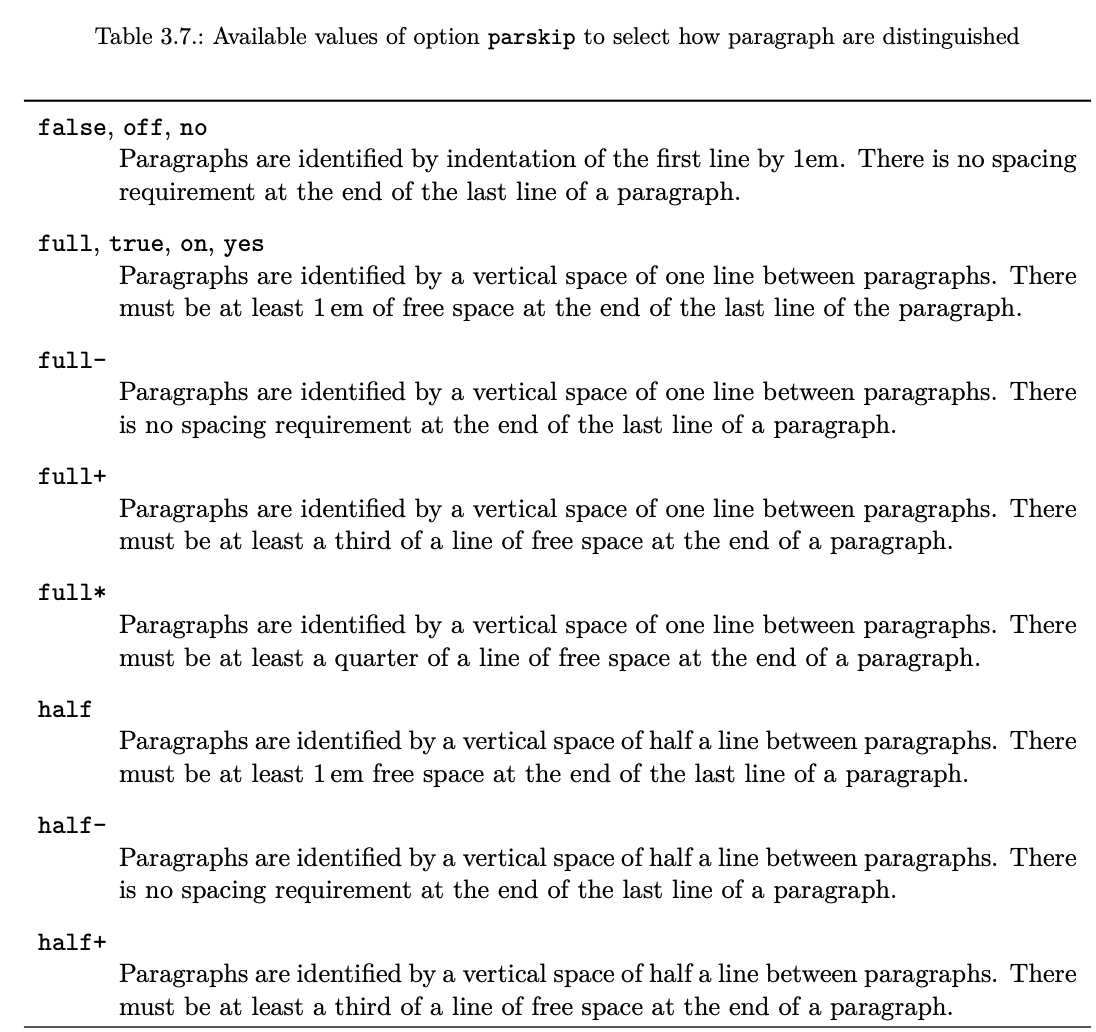
\includegraphics[width=0.9\linewidth]{imagens/tab3_7.png}
    \caption{Tabela 3.7 do Manual}
    \label{fig:tab3_7}
\end{figure}

\begin{figure}[hb]
    \centering
    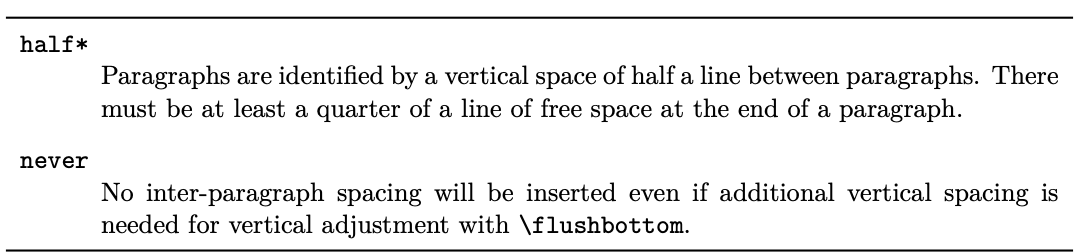
\includegraphics[width=0.9\linewidth]{imagens/tab3_7b.png}
    \caption{Tabela 3.7 do Manual}
    \label{fig:tab3_7b}
\end{figure}

Todos os oito valores de opção \texttt{full} e \texttt{half} também alteram o espaçamento antes, depois e dentro dos ambientes de lista. Isso impede que esses ambientes ou os parágrafos dentro deles tenham uma separação maior do que aquela entre os parágrafos do texto normal. Além disso, essas opções garantem que o índice e as listas de figuras e tabelas sejam definidos sem nenhum espaçamento adicional.

O comportamento padrão do \KOMAScript\ é \texttt{parskip=false}. Nesse caso, não há espaçamento entre parágrafos, apenas um recuo da primeira linha por 1em.
